\documentclass{article}

\usepackage[margin=3cm]{geometry}
\usepackage{amsmath}
\usepackage{amsfonts}
\usepackage{amssymb}
\usepackage{amscd}
\usepackage{standalone}
\usepackage{float}
\usepackage{color}
\usepackage[shortlabels]{enumitem}
\usepackage{graphicx}
\usepackage{caption}
\usepackage[ngerman]{babel}
\usepackage{lscape}
\usepackage{cancel}
\usepackage{dirtytalk}
\usepackage{siunitx}
\usepackage{listings}

\graphicspath{ {./images/} }

\begin{document}
\begin{titlepage}
    \centering
    {\scshape\LARGE Hochschule für Technik und Wirtschaft Dresden \par}
    \vspace{1cm}
    {\scshape\Large Softwaresystem \glqq GPS-Track-App\grqq\par}
    \vspace{1.5cm}
    {\huge\bfseries Betriebsanleitung\par}
    \vspace{2cm}
    {\Large\itshape Raphael Neubert, Alexander Pronin \par}
    \vfill

    {\large \today\par}
\end{titlepage}

\tableofcontents
\newpage

\section{Server}
Der Server stellt eine REST-API zur Verfügung mit der sich GPS-Track auf dem Server 
speichern und herunterladen lassen.
\subsection{Allgemeiner Aufbau}
Der Server besteht aus einer einzigen Python-Datei.
Die GPS-Tracks werden in einen Ordner \say{files} gespeichert,
welcher sich (standartmäßig) im Pfad der Python-Datei befinden muss.
Der Ort an dem die GPS-Tracks gespeichert werden kann in der Python-Datei
angepasst werden. \\ \par
\textbf{Endpunkte:}
\begin{itemize}
    \item \textit{/} \\ Website zur Überprüfung, ob der Server online ist.
    \item \textit{/liste} \\ Ermöglicht es mithilfe von GET-Request eine Liste
        mit den, auf dem Server vorhandenen Dateien, zu erhalten.
    \item \textit{/dellist} \\ Ermöglicht es 
        mithilfe von GET-Request eine Liste
        mit den, vom Server gelöschten Dateien, zu erhalten.
    \item \textit{/upload} \\  Ermöglicht es mithilfe von POST-Requests GPS-Tracks 
        auf den Server zu laden.
    \item \textit{/download/}$<$\textit{path:filename}$>$ \\  Ermöglicht es mithilfe
        von GET-Requests GPS-Tracks vom Server zu laden.
    \item \textit{/delete/}$<$\textit{path:filename}$>$  \\
        Ermöglicht es mithilfe von GET-Requests GPS-Tracks 
        vom Server zu löschen. Falls die Datei \say{./delete.txt} auf dem Server noch
        nicht existiert, wird diese erzeugt. Der Datei \say{./delete.txt} wird 
        der Name der durch den Request gelöschte Datei, angehangen.
\end{itemize}
\subsection{Anforderungen}
Der Server ist minimalistisch gehalten. Daher ist ein System mit wenig 
Leistung z.B. ein Raspberry Pi ausreichend. Es sollte sichergestellt 
werden, dass auf dem Server genügen Speicherplatz für die gewünschte Anzahl an 
GPS-Tracks vorhanden ist. Auf dem System muss ein Python3 Interpreter, sowie das 
Python-Framework Flask installiert sein.
\subsection{Installation}
\subsubsection{Debian}
Die folgenden Schritte gelten nicht nur für Debian selber, sondern auch für andere 
Linux-Distributionen die den Packetmanager \say{apt} verwenden. (z.B. Ubuntu, Mint)\par

\begin{enumerate}
    \item Installation der benötigten Programme: 
        \begin{itemize}
            \item Updaten des Betriebssytems sowie alle auf dem System 
                installierten Bibliotheken. \\
                \textit{sudo apt update} \\
                \textit{sudo apt upgrade}
            \item Installation von Python3 sowie den Python3-Packagemanger \say{pip3} \\
                \textit{sudo apt install python3} \\
                \textit{sudo apt install python3-pip}\\
                \textit{sudo apt install cron}
        \end{itemize}
    \item Installation der benötigten Python-Frameworks: 
        \begin{itemize}
            \item Installation von \say{Flask} mithilfe von \say{pip3} \\
                \textit{pip3 install flask}
        \end{itemize}
    \item Manuelles Starten des Servers: \\
        \textit{python3 app.py} 
    \item Automatisches Starten des Python-Programms beim Hochfahren des Servers: \\ 
        Kann auf verschieden realisiert werden (z.B. SystemD, OpenRC).
        Hier: mithilfe von \say{Cronjobs}.  \\
        \textit{crontab -e} \\ 
        Falls \say{Crontab} zum ersten mal ausgeführt wurde muss nun ein Editor gewählt
        werden. Anschließend muss folgende Zeile an das ende der nun offenen Datei 
        angehangen werden. \\
        \say{@reboot cd $<$path$>$ \&\& python3 app.py}
\end{enumerate}
\subsubsection{andere Betriebssysteme}
\begin{itemize}
    \item Die Installation auf andern Linux-basierten Betriebssystemen erfolgt
        fast identisch. Lediglich die Befehle zur Installation
        der Programme können anders sein.
    \item Die Installation auf Windows ist möglich und kann am einfachsten 
        unter Verwendung eines \say{Virtual Environments} realisiert werden. Dies 
        wird hier aber nicht weiter erläutert.
\end{itemize}
\subsection{Wartung}
Im Normalfall bedarf der Server keinerlei Wartung. 
Es sollte jedoch sichergestellt werden, dass das Betriebssystem regelmäßig aktualisiert
wird. Sollte nach langem Betrieb die Synchronisation lange dauern oder eine 
hohe Netzauslastung verursachen, kann es daran liegen, dass auf dem Server
die datei \say{./delete.txt} zu groß geworden ist. Wenn alle Endgeräte auf dem 
gleichen Synchronisationsstand sind, kann diese Problemlos gelöscht werden.
\section{App}
\subsection{Anforderungen}
\subsubsection{für das Kompilieren}
Das Programm \say{Android Studio}. Es ist auch möglich die App ohne Android Studio, direkt mit \say{gradlew} zu Kompilieren.
In dieser Anleitung wird jedoch nur ersteres gezeigt. Entwickelt wurde die App mit \say{Android Studio 2021.2.1}, die
verschiedenen Android Studio Versionen weisen aber eine hohe Kompatibilität auf weshalb auch andere Versionen
problemlos funktionieren sollten.
\subsubsection{für die Installation}
Damit die App vollständig Funktioniert muss sich auf dem Smartphone mindestens Android 8 (API level 29) befinden.
Falls dies nicht der Fall ist kann die App trotzdem installiert werden (solange mindestens API level 26 unterstützt wird)
es gibt jedoch Einschränkungen bei den Funktionalitäten. Zum Beispiel ist dann eine Aufnahme im Hintergrund nicht mehr
möglich.
\subsection{Building}
\begin{enumerate}
    \item Nach der erstmaligen Installation muss zunächst Android Studio eingerichtet werden.

        \begin{minipage}{0.5\textwidth}
        \begin{figure}[H]
            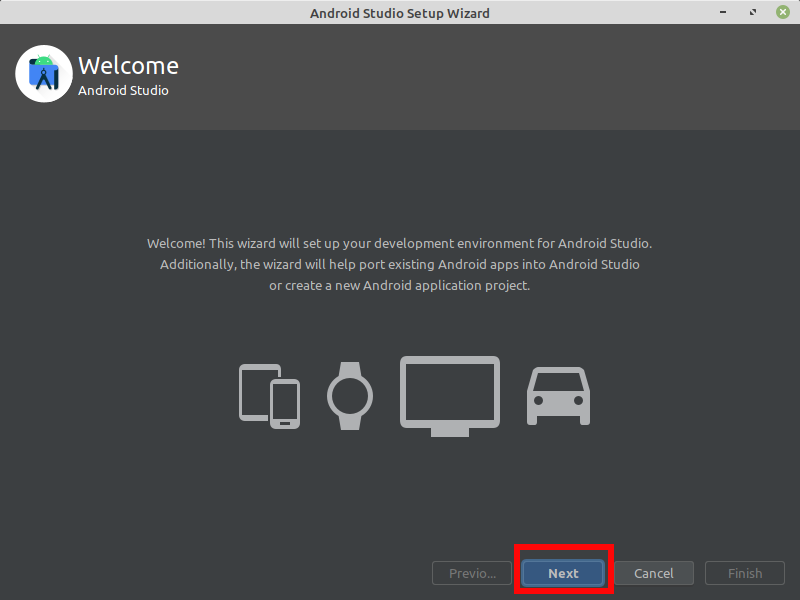
\includegraphics[scale=0.27]{1.png}
        \end{figure}
        \begin{figure}[H]
            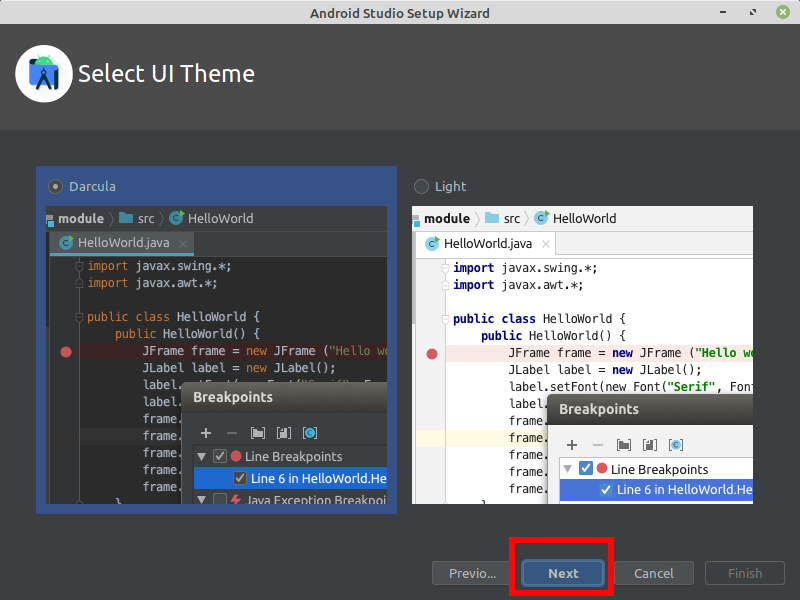
\includegraphics[scale=0.27]{3.png}
        \end{figure}
        \begin{figure}[H]
            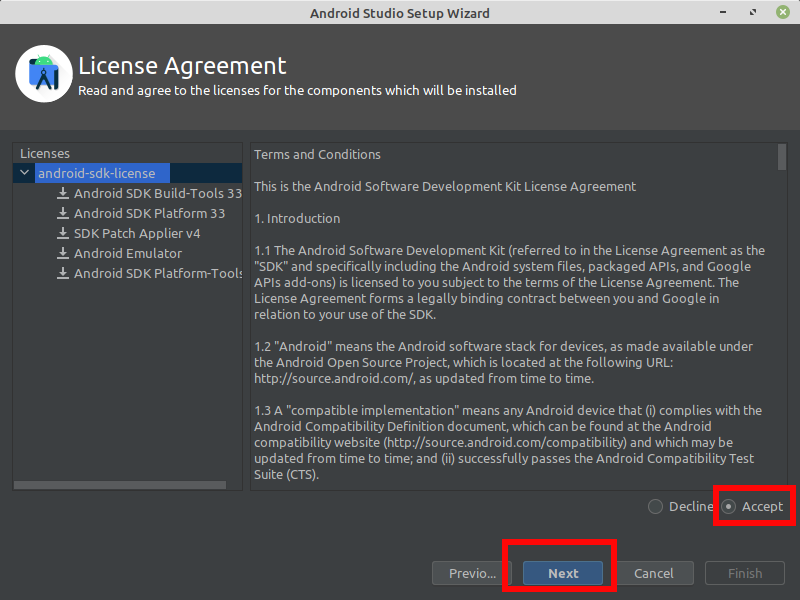
\includegraphics[scale=0.27]{5.png}
        \end{figure}
        \end{minipage}
        \begin{minipage}{0.5\textwidth}
        \begin{figure}[H]
            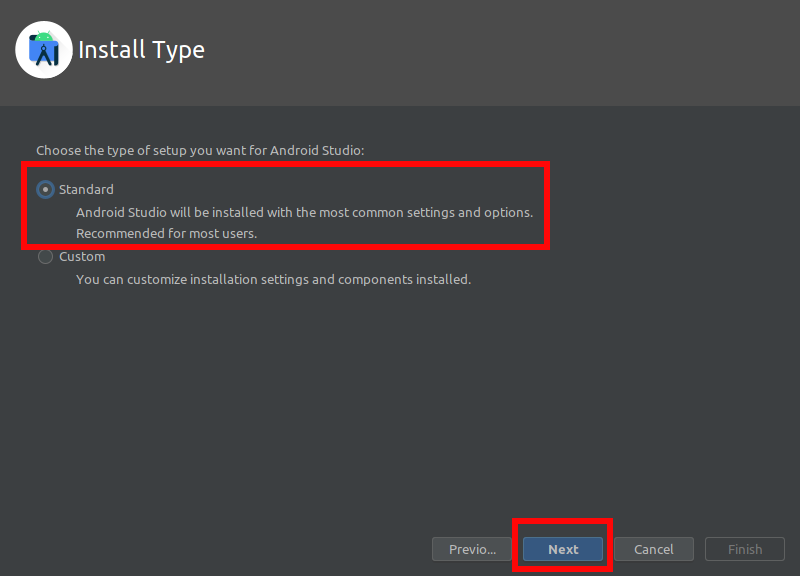
\includegraphics[scale=0.28]{2.png}
        \end{figure}
        \begin{figure}[H]
            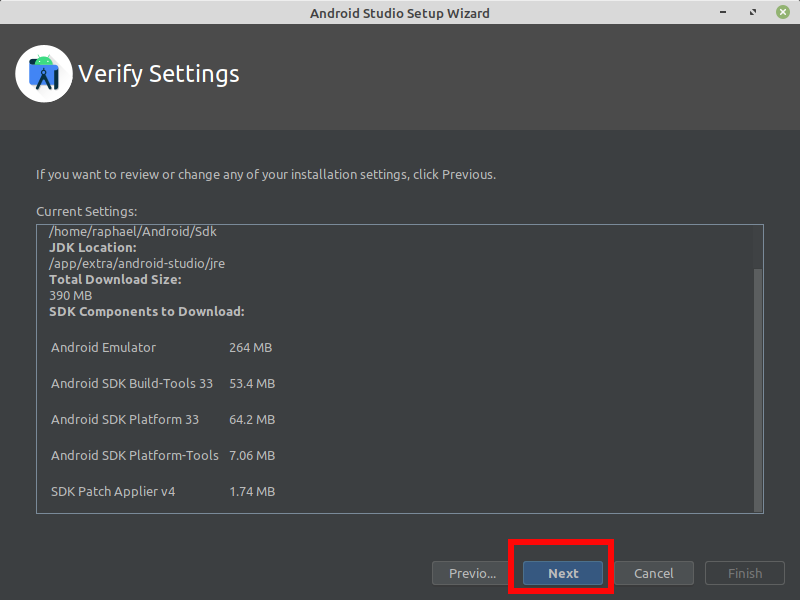
\includegraphics[scale=0.27]{4.png}
        \end{figure}
        \begin{figure}[H]
            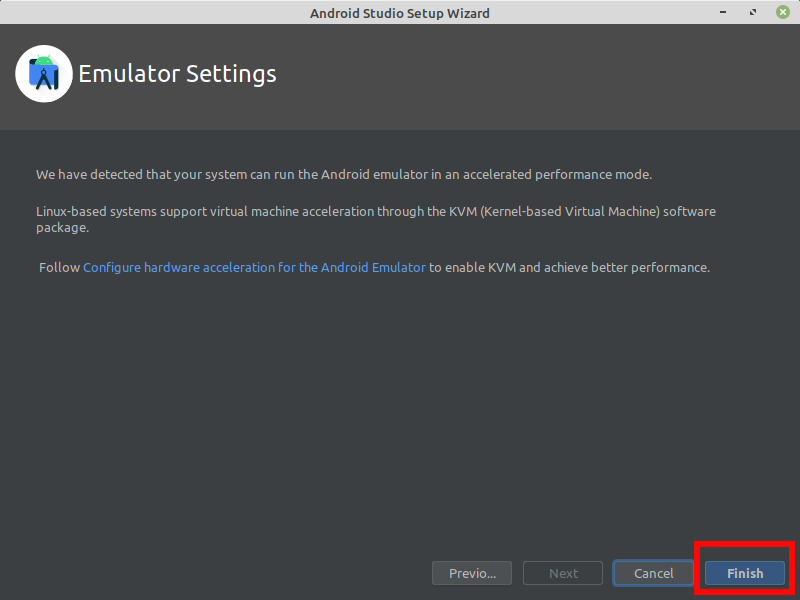
\includegraphics[scale=0.27]{6.png}
        \end{figure}
        \end{minipage}
        
        \begin{figure}[H]
            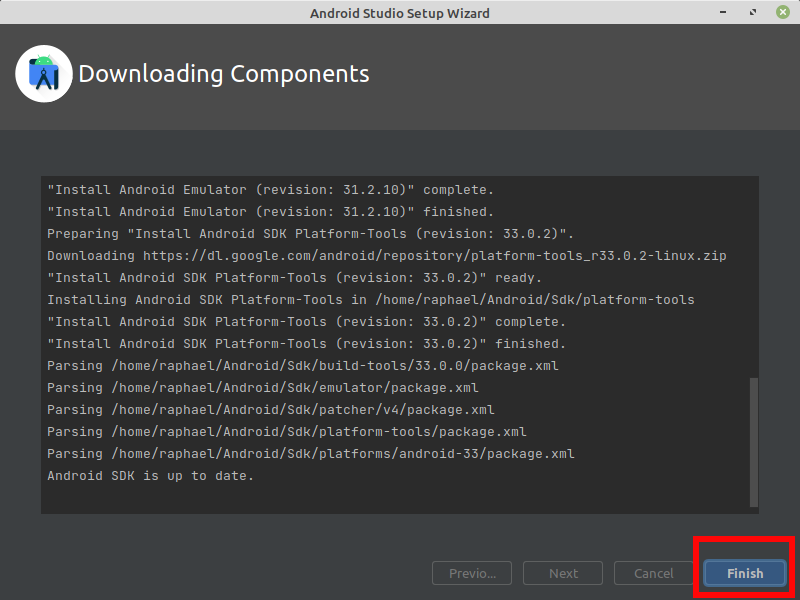
\includegraphics[scale=0.3]{7.png}
            \centering
        \end{figure}

    \item Jetzt kann das Projekt geöffnet werden. Beim Öffnen werden automatisch alle benötigten Bibliotheken und Tools
        installiert deshalb kann es einen Moment dauern.

        \begin{minipage}{0.6\textwidth}
        \begin{figure}[H]
            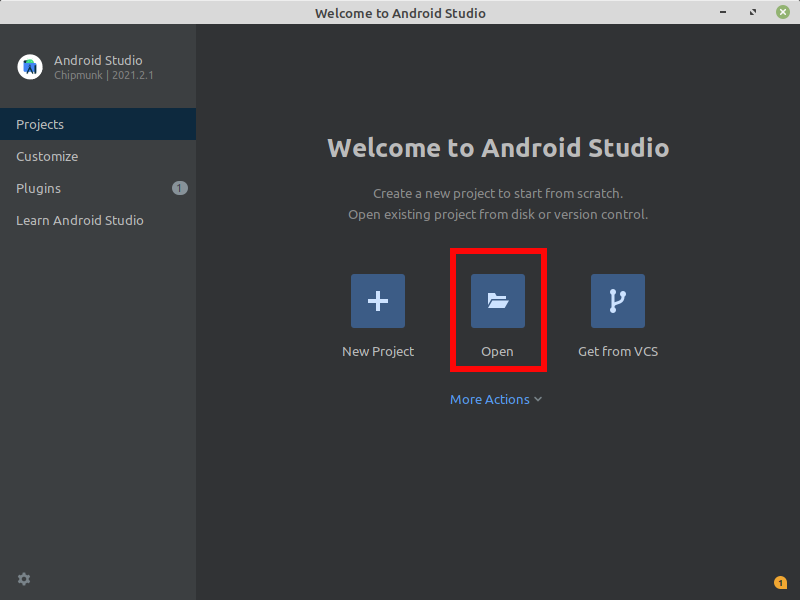
\includegraphics[scale=0.3]{8.png}
        \end{figure}
        \end{minipage}
        \begin{minipage}{0.4\textwidth}
        \begin{figure}[H]
            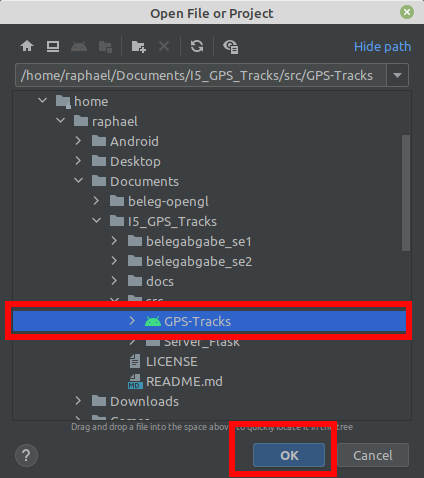
\includegraphics[scale=0.38]{9.png}
        \end{figure}
        \end{minipage}
        
        \begin{figure}[H]
            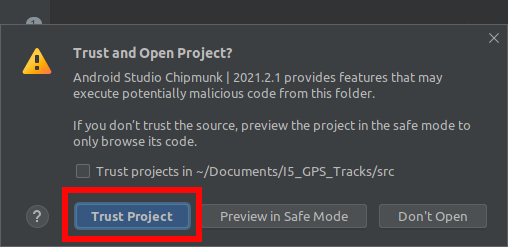
\includegraphics[scale=0.4]{10.png}
            \centering
        \end{figure}
    \item Anschließend kann die App mit der Tastenkombination STRG+F9 oder über das Menu \say{Build} kompiliert werden.
        \newpage
    \item Erzeugung einer signierten APK (Nur signierte APK's können auf Android-Geräten installiert werden).
        \begin{enumerate}
            \item Auswahl der Option \say{Generate Signed Bundle / APK...} im Menu \say{Build}.
            \item Auswahl der Option \say{APK}
                \begin{figure}[H]
                    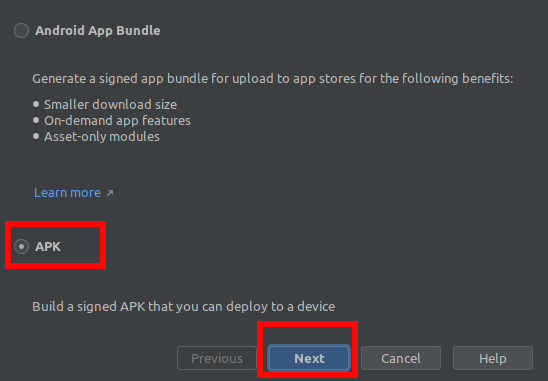
\includegraphics[scale=0.4]{11.png}
                    \centering
                \end{figure}
            \item Erzeugung eines \say{Keystores} sowie des Schlüssels zum Signieren der APK.
                \begin{figure}[H]
                    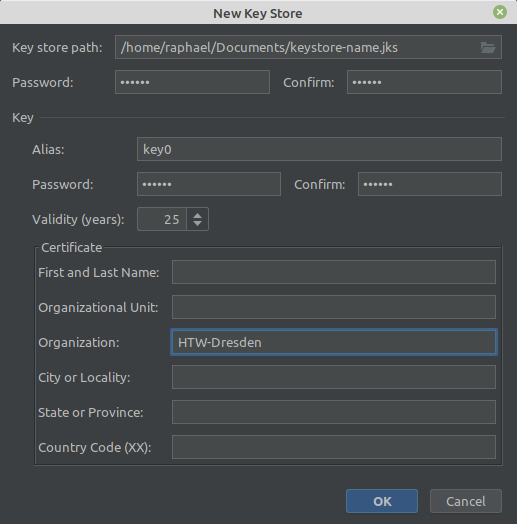
\includegraphics[scale=0.4]{12.png}
                    \centering
                \end{figure}
                Es ist ausreichend wenn eines der \say{Certificate} Felder ausgefüllt ist.
                \newpage
            \item Auswahl der Build-Variante.
                \begin{figure}[H]
                    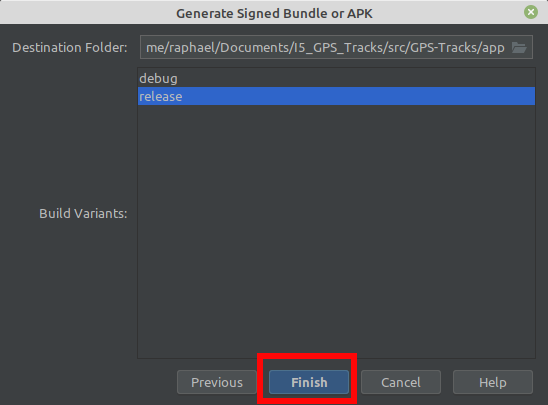
\includegraphics[scale=0.4]{13.png}
                    \centering
                \end{figure}
        \end{enumerate}
        Die Erzeugte APK befindet sich nun im Pfad der App unter \say{./app/release/}.
\end{enumerate}

\subsection{Installation}
\subsubsection{per APK}
Bei der Installation per APK kann es je nach Android-Version kleine Unterschiede geben.
\begin{enumerate}
    \item Öffnen des Dateiexplorers, Navigation zur APK und Auswahl dieser.
        \begin{figure}[H]
            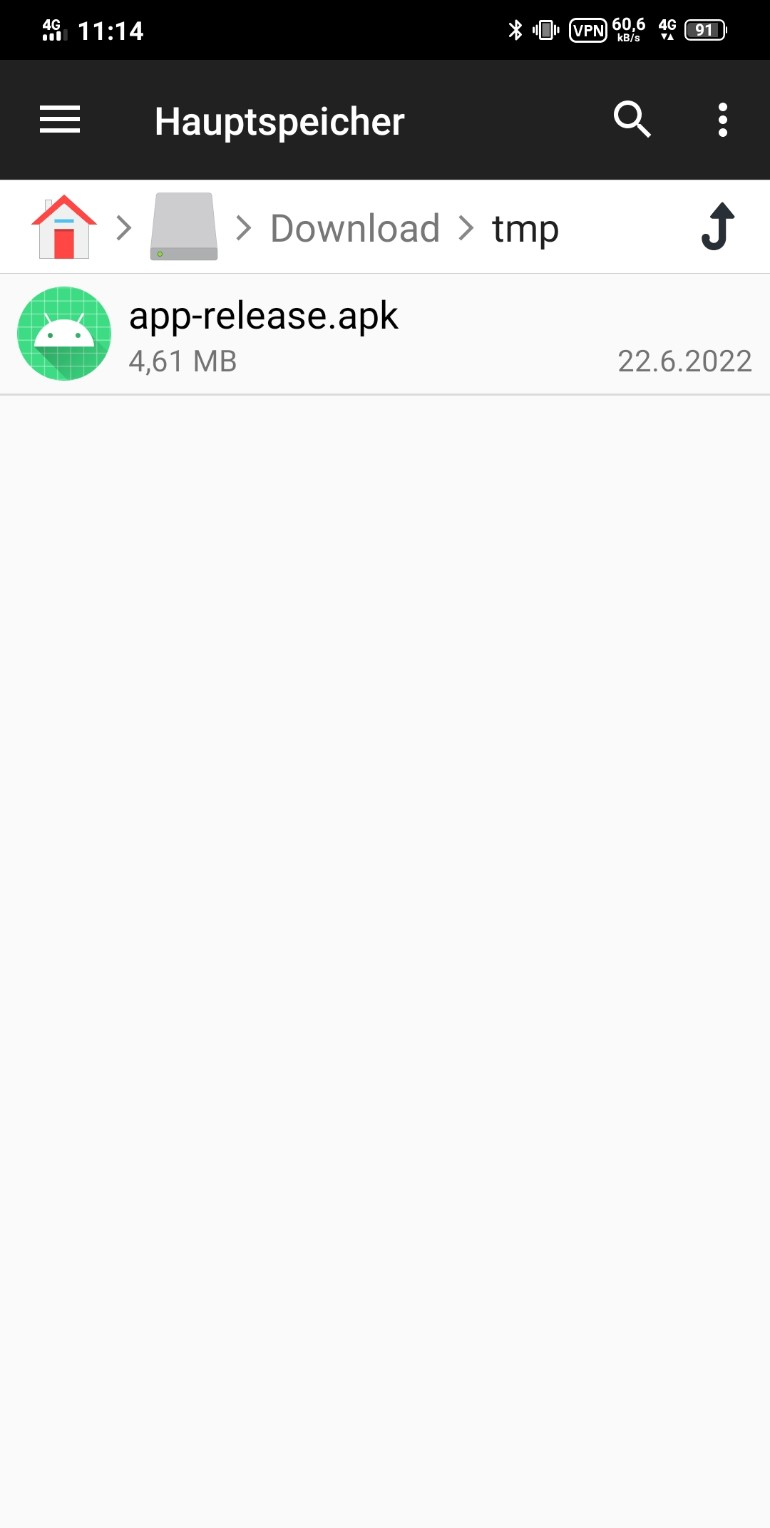
\includegraphics[scale=0.2]{14.jpg}
            \centering
        \end{figure}
    \item Falls mehrere Programme zum Öffne zur Auswahl stehen, das Programm \say{Paketinstallation} wählen.
        \begin{figure}[H]
            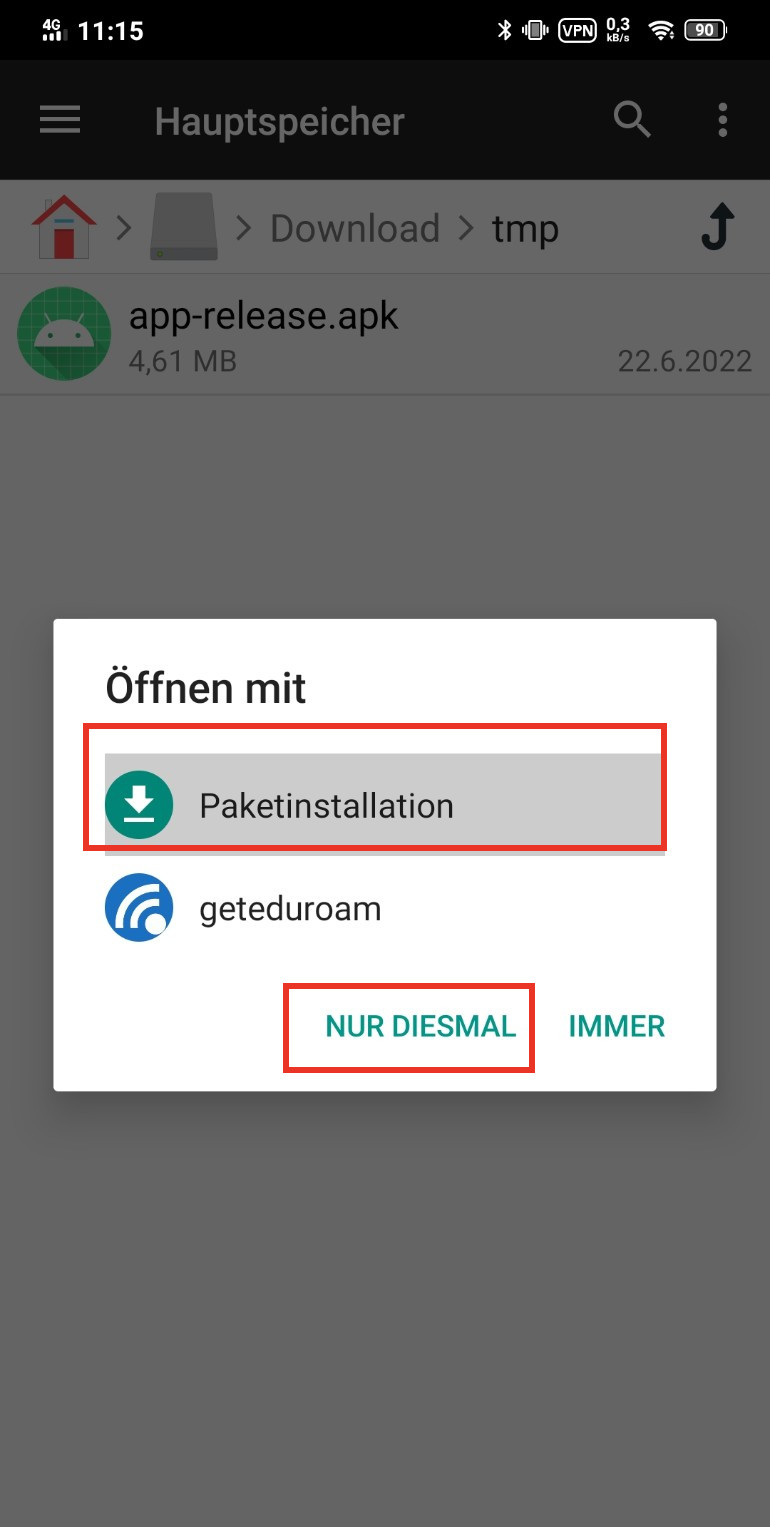
\includegraphics[scale=0.6]{15.jpg}
            \centering
        \end{figure}
    \item Dem Dateiexplorer muss nun gegebenenfalls die Berechtigung, zur Installation von Apps gegeben werden.

        \begin{minipage}{0.5\textwidth}
        \begin{figure}[H]
            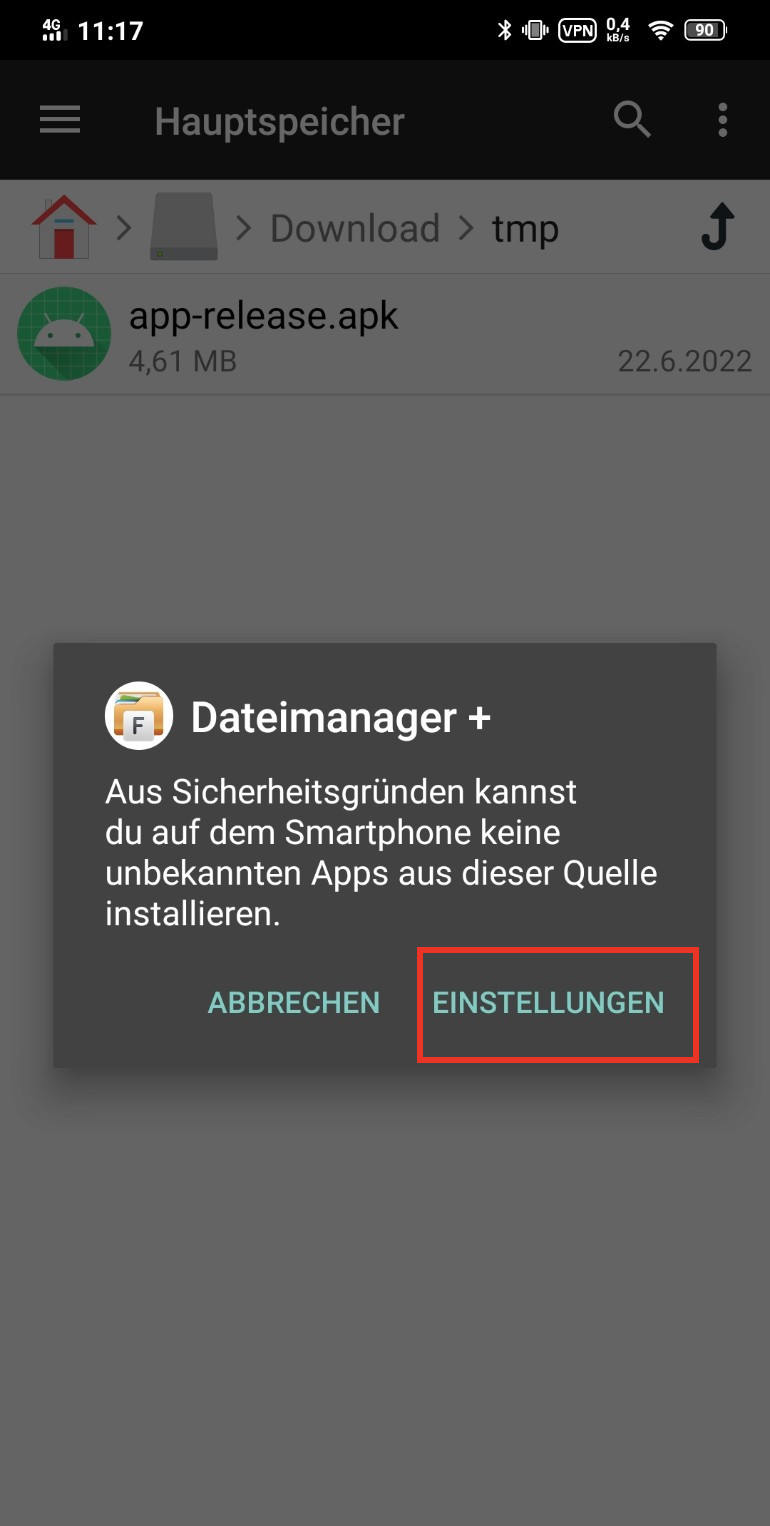
\includegraphics[scale=0.85]{16.jpg}
            \centering
        \end{figure}
        \end{minipage}
        \begin{minipage}{0.5\textwidth}
        \begin{figure}[H]
            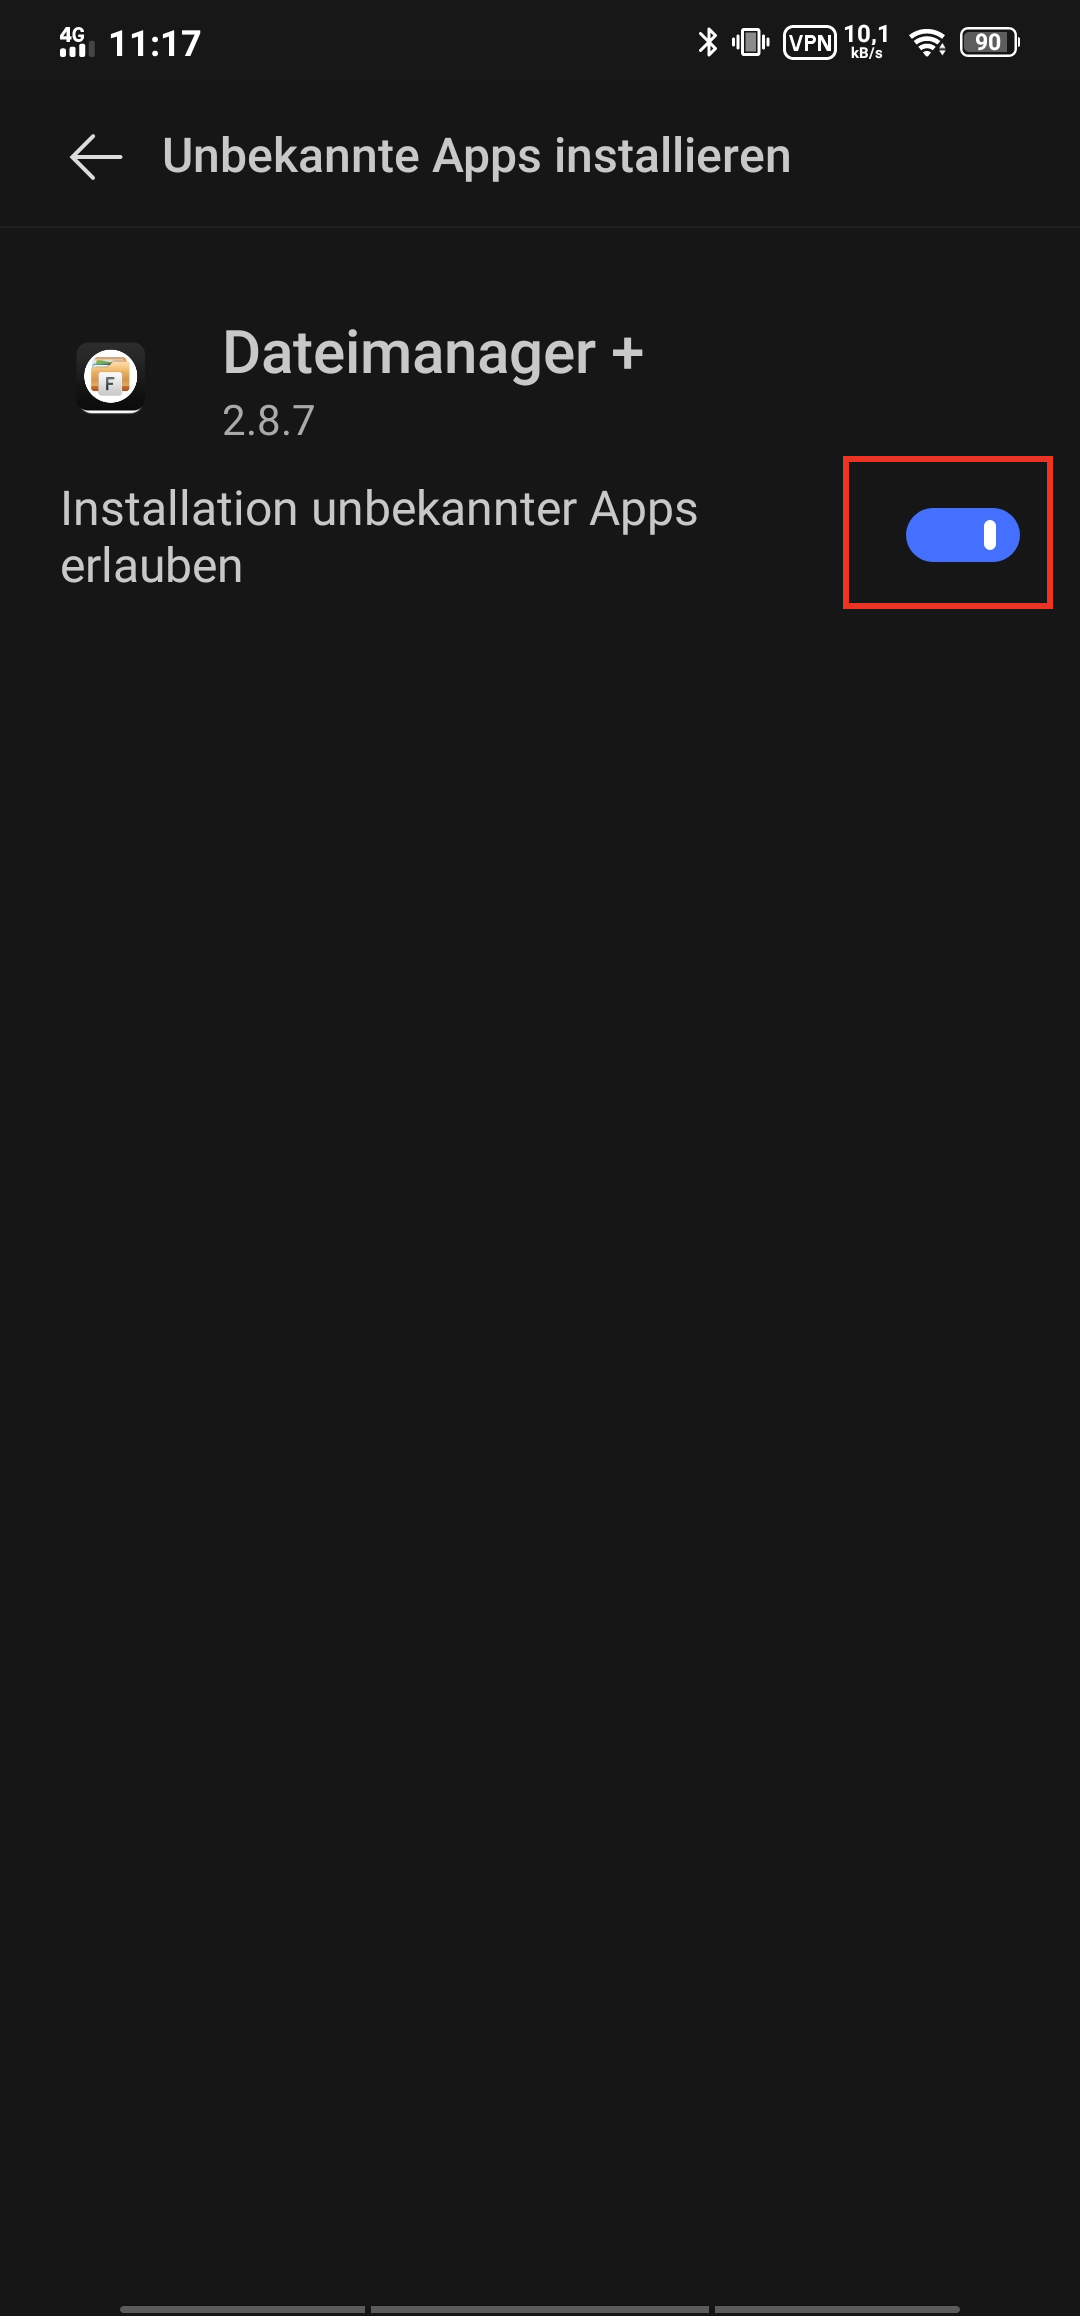
\includegraphics[scale=0.56]{17.jpg}
            \centering
        \end{figure}
        \end{minipage}
        
    \item Anschließend kann die App installiert werden.

        \begin{minipage}{0.5\textwidth}
        \begin{figure}[H]
            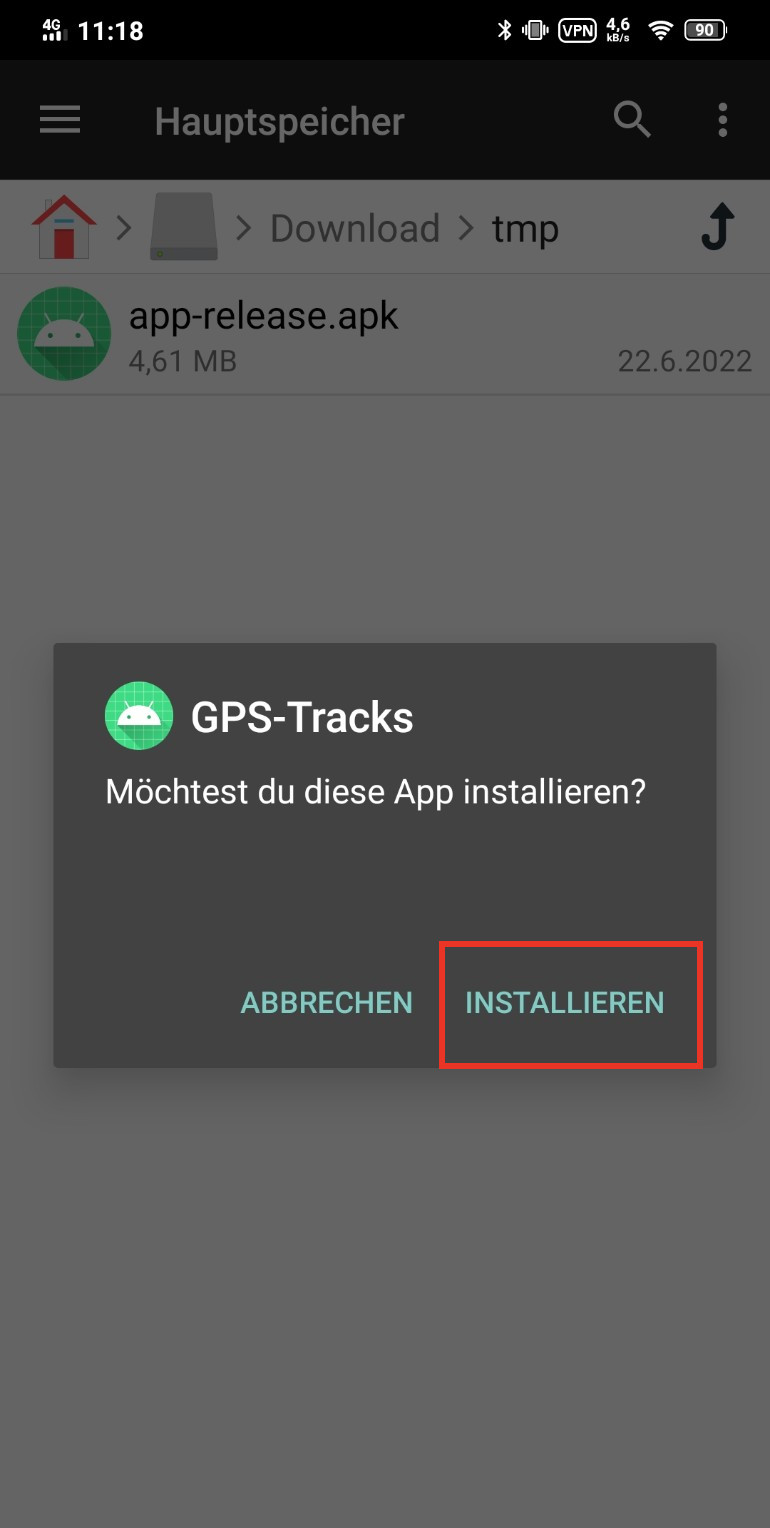
\includegraphics[scale=0.81]{18.jpg}
            \centering
        \end{figure}
        
        \end{minipage}
        \begin{minipage}{0.5\textwidth}
        \begin{figure}[H]
            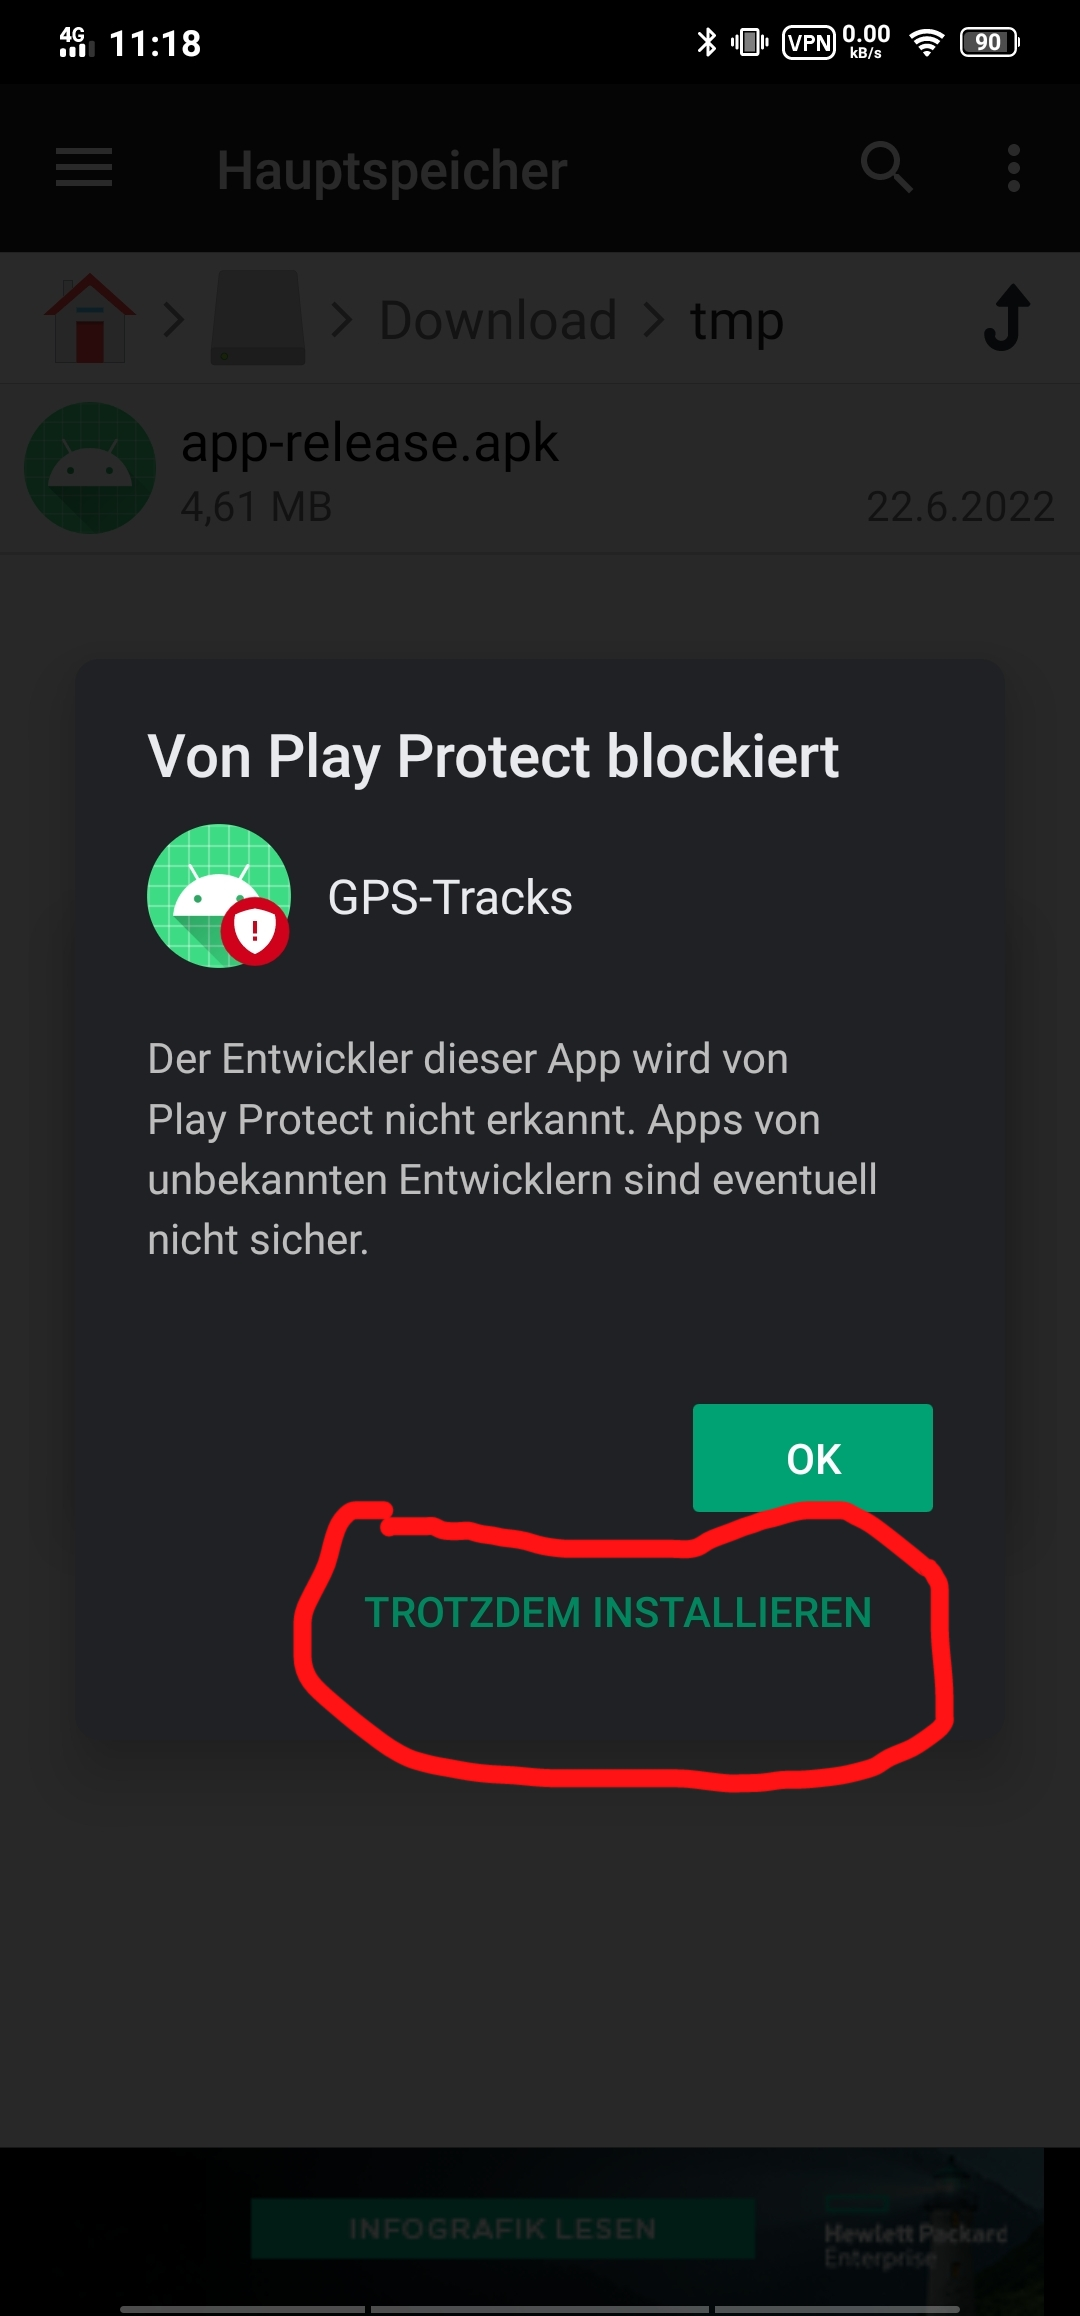
\includegraphics[scale=0.13]{19.jpg}
            \centering
        \end{figure}
        \end{minipage}
        
        \begin{figure}[H]
            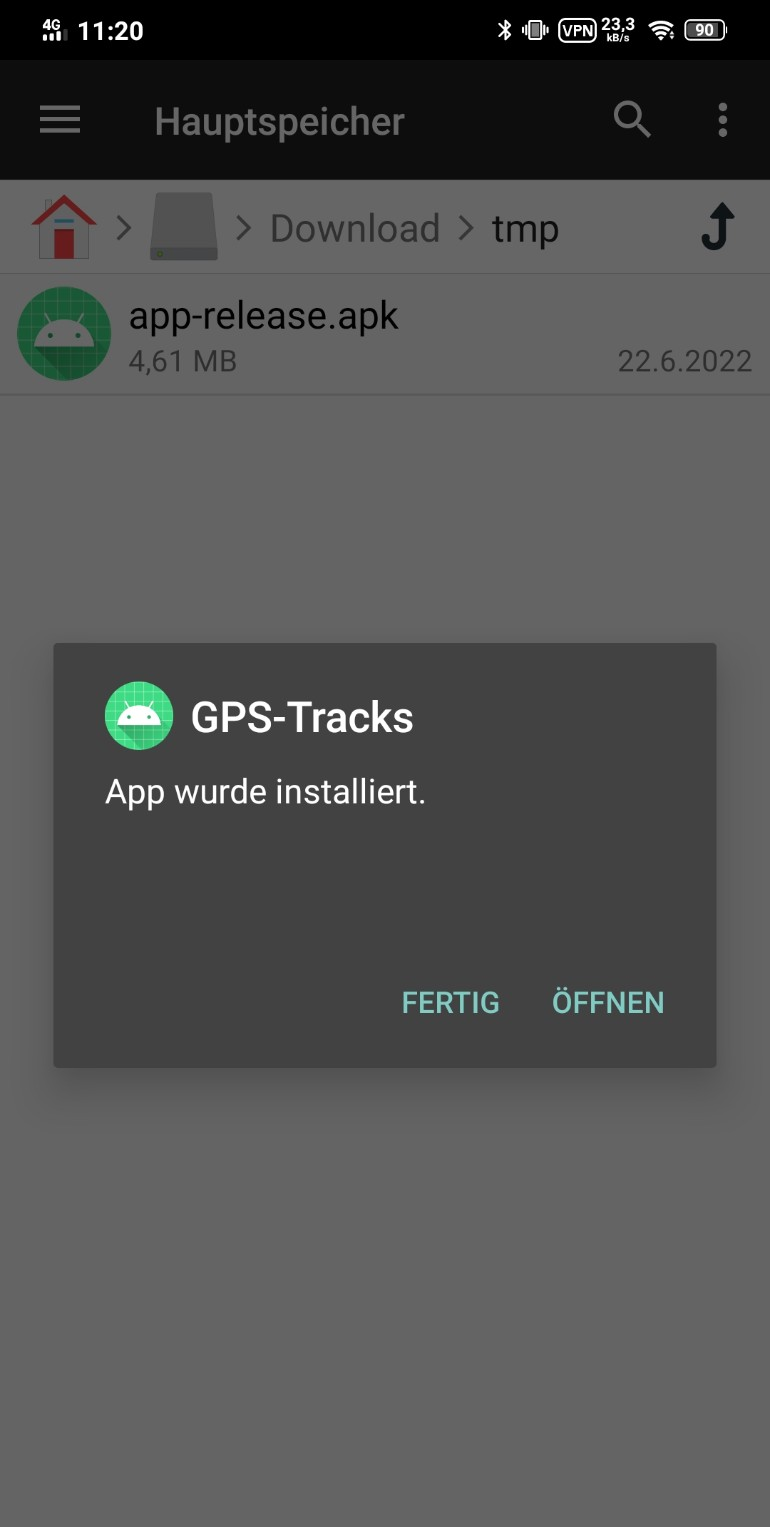
\includegraphics[scale=0.18]{20.jpg}
            \centering
        \end{figure}
\end{enumerate}
\subsubsection{über Android Studio}
Alternativ zur Installation per APK, ist es auch möglich die App über Android Studio zu installieren. 
Die App lässt sich sowohl auf einem Emulator als auch einem echten Smartphone installieren.
Die zur Installation nötigen Schritte sind dabei fast identisch. Ist eine Installation auf einem Emulator erwünscht,
muss dieser allerdings noch erstellt werden. Dies kann im Tab \say{Device Manager} (am rechten Rand) getan werden.
\begin{enumerate}
    \item Anschließen des Smartphones an den PC bzw. starten des Emulators.
    \item Falls es sich um ein echtes Smartphone handelt muss nun auf diesem das \say{USB-Debugging} erlaubt werden.
        \begin{figure}[H]
            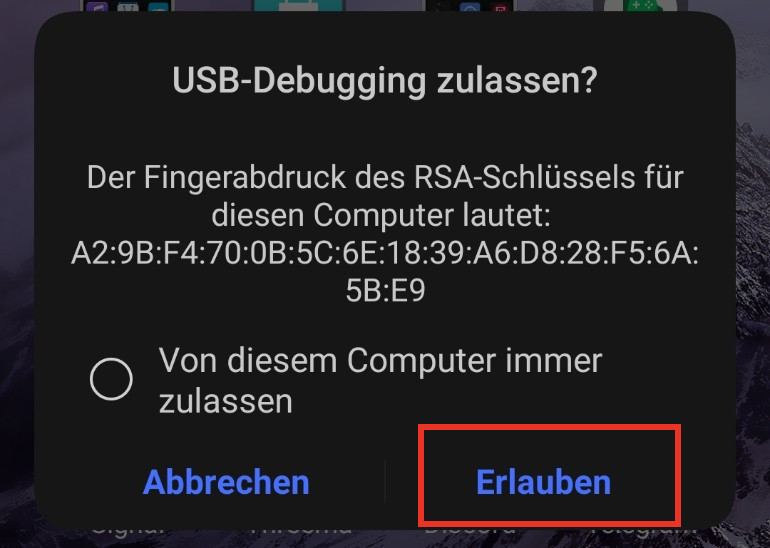
\includegraphics[scale=0.8]{21.jpg}
            \centering
        \end{figure}
    \item Mit einem Klick auf den grünen Play-Button kann jetzt die App installiert und gestartet werden. 
        \begin{figure}[H]
            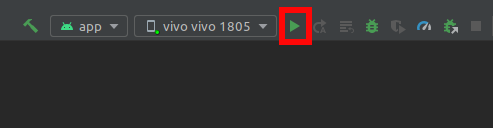
\includegraphics[scale=0.6]{22.png}
            \centering
        \end{figure}
\end{enumerate}
\textbf{Achtung:} Auf diese Art und Weise installiert man lediglich die Debug-Version der App. Falls die release-Version 
per Android Studio installiert werden soll muss dies in den Build-Optionen spezifiziert werden.
\end{document}
